\section{Cloud, Wilderness, and River}
\label{sec:cloud-wilderness-jordan}

The Book of Exodus closes not with a human ceremony of praise, but with a sudden silence that stops even Moses at the door. ``So in the first month of the second year, the first day of the month, the tabernacle was set up'' (Exod 40:15). Moses raises the acacia boards on their silver sockets, lays the testimony inside the Ark, sets the golden propitiatory above it, draws the inner veil across the Holy of Holies, arranges the table, the seven-branched lampstand, and the incense altar in the outer chamber, and sets the bronze laver and altar of holocausts in the courtyard. Every command given on Mount Sinai has been answered in obedience. The instant Moses finishes the work, heaven takes possession of the dwelling:

\begin{quote}
The cloud covered the tabernacle of the testimony, and the glory of the Lord filled it. Neither could Moses go into the tabernacle of the covenant, the cloud covering all things, and the majesty of the Lord shining, for the cloud had covered all. If at any time the cloud removed from the tabernacle, the children of Israel went forward by their troops: If it hung over, they remained in the same place. For the cloud of the Lord hung over the tabernacle by day, and a fire by night, in the sight of all the children of Israel throughout all their mansions. (Exod 40:32--36 [Hebrew/LXX 40:34--38])
\end{quote}

Moses had walked through the Red Sea, climbed Sinai amid thunder, and spoken with God as a man speaks to his friend. Yet when the glory of the Lord descends upon the completed Tent and fills the inner chamber where the Ark rests, even Moses cannot cross the threshold. The sanctuary is no longer merely a well-ordered work of Israelite craft; it has become the consecrated habitation of the living God, veiled by cloud by day and blazing with fire by night before the eyes of every tribe.

\subsection{The Cloud Overshadows the Tent}
\label{subsec:cloud-overshadows-tent}

A precious textual detail in these closing verses of Exodus links the wilderness Tabernacle directly to the chamber of Nazareth. Because the Vulgate and Douay-Rheims omit two verses earlier in chapter 40, the cloud's descent stands at Exodus 40:32--36 in the Latin and Douay-Rheims numbering and at Exodus 40:34--38 in the Hebrew and Greek Septuagint. Within that descent, the Clementine Vulgate describes the cloud covering the Tent with forms of the Latin verb \textit{operio} (``to cover''): \textit{operuit} (``covered''), \textit{nube operiente omnia} (``the cloud covering all things''), and \textit{operuerat} (``had covered''). The Greek Septuagint, however---rendered verbatim in Brenton's English translation of Exodus 40:35---uses the language of overshadowing:

\begin{quote}
And Moses was not able to enter into the tabernacle of testimony, because the cloud overshadowed it, and the tabernacle was filled with the glory of the Lord.
\end{quote}

That Septuagint idiom of the divine cloud \textit{overshadowing} (\textit{episkiazo}) the dwelling recurs throughout Numbers 9--10 whenever the cloud rests over the Tabernacle or moves with Israel on the march (Num 9:18, 20, 22; 10:36 in Brenton's Septuagint). In the Greek Psalter, Psalm 90:4 pairs the exact future verbal phrase \textit{episkiasei soi} (``he shall overshadow thee,'' Vulgate \textit{obumbrabit tibi}) with the shelter of God's wings---evoking the outstretched cherubim above the Ark. At the Annunciation, the Archangel Gabriel speaks those exact words to the Virgin of Nazareth: ``The Holy Ghost shall come upon thee and the power of the Most High shall overshadow thee. And therefore also the Holy which shall be born of thee shall be called the Son of God'' (Luke 1:35; Greek \textit{episkiasei soi}, Vulgate \textit{obumbrabit tibi}).

Commentators across Catholic tradition read that overshadowing cloud as a veil drawn over an unsearchable divine work. In his \textit{Commentary on the Gospel of Luke} on 1:35, Cornelius a Lapide explains Gabriel's promise in words that echo Moses standing outside the filled Tent at Sinai:

\begin{quote}
It will cover thee as with a veil, i.e., will secretly work a mighty operation in thee; for it will be such and so great a one that no man or angel can penetrate into or comprehend it.
\end{quote}

The Tabernacle itself teaches this same reverence through its nested east-to-west gradation of holiness (Exod 26--27; 30:17--21; 40:1--36). A wide white linen enclosure separates the sacred precinct from the surrounding Israelite camp, opened by a single embroidered gate on the east. Entering that courtyard, a worshipper encounters bronze: first the square horned altar of burnt offering, where daily sacrifice is offered, and behind it the bronze laver, where Aaron and his sons wash hands and feet before serving. Beyond the laver stands the veiled Tent of Meeting, divided internally into two chambers. In the outer room, called the Holy Place (\textit{Sancta}), priests enter daily to tend the seven-branched golden lampstand, the golden table of the loaves of proposition, and the golden altar of incense standing directly before the inner curtain (Heb 9:2, 6). Beyond that embroidered inner veil lies the Most Holy Place (\textit{Sancta sanctorum}), an unlit cube holding the Ark of the Covenant alone, into which the high priest alone enters once a year on the Day of Atonement, not without blood (Heb 9:3, 7). Every step westward moves from bronze to gold, from daily sacrifice to perpetual incense, and from priestly ministry to the silent cloud resting above the mercy seat.

\ifdefined\TriptychPrintEdition
\Needspace{24\baselineskip}
\begin{center}
\begin{tikzpicture}
  \node[anchor=south west, inner sep=0] (img) at (0,0) {%
    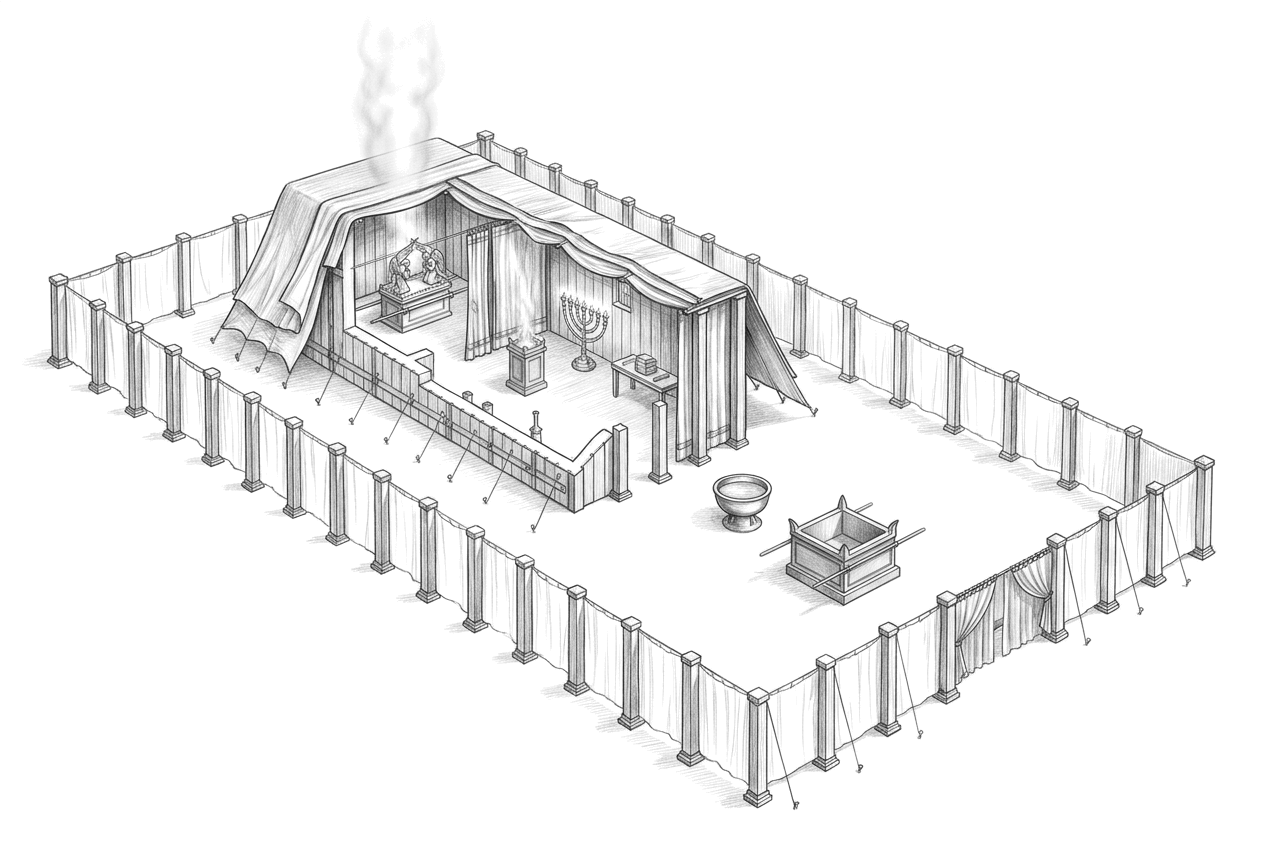
\includegraphics[width=0.92\linewidth]{theology/mariology/ark-of-the-covenant/artwork/tabernacle-sanctuary-graphite.png}%
  };
  \begin{scope}[x={(img.south east)}, y={(img.north west)}]
    \node[font=\scriptsize, fill=white, inner sep=1.5pt] (t1) at (0.15, 0.91) {Cloud of the divine presence};
    \draw[draw=black!65, line width=0.4pt] (t1) -- (0.29, 0.87);
    \fill[black!75] (0.29, 0.87) circle (1.1pt);

    \node[font=\scriptsize, fill=white, inner sep=1.5pt] (t2) at (0.52, 0.91) {Most Holy Place and Ark};
    \draw[draw=black!65, line width=0.4pt] (t2) -- (0.33, 0.70);
    \fill[black!75] (0.33, 0.70) circle (1.1pt);

    \node[font=\scriptsize, fill=white, inner sep=1.5pt] (t3) at (0.63, 0.82) {Inner veil};
    \draw[draw=black!65, line width=0.4pt] (t3) -- (0.385, 0.69);
    \fill[black!75] (0.385, 0.69) circle (1.1pt);

    \node[font=\scriptsize, fill=white, inner sep=1.5pt] (t4) at (0.80, 0.72) {Holy Place};
    \draw[draw=black!65, line width=0.4pt] (t4) -- (0.48, 0.60);
    \fill[black!75] (0.48, 0.60) circle (1.1pt);

    \node[font=\scriptsize, fill=white, inner sep=1.5pt] (t5) at (0.22, 0.19) {Bronze laver};
    \draw[draw=black!65, line width=0.4pt] (t5) -- (0.57, 0.39);
    \fill[black!75] (0.57, 0.39) circle (1.1pt);

    \node[font=\scriptsize, fill=white, inner sep=1.5pt] (t6) at (0.35, 0.10) {Altar of burnt offering};
    \draw[draw=black!65, line width=0.4pt] (t6) -- (0.65, 0.33);
    \fill[black!75] (0.65, 0.33) circle (1.1pt);

    \node[font=\scriptsize, fill=white, inner sep=1.5pt] (t7) at (0.86, 0.13) {East court entrance};
    \draw[draw=black!65, line width=0.4pt] (t7) -- (0.79, 0.27);
    \fill[black!75] (0.79, 0.27) circle (1.1pt);
  \end{scope}
\end{tikzpicture}
\end{center}\nopagebreak[4]
\else
\begin{studybox}{Plate II: The Wilderness Tabernacle and Nested Gradation of Holiness}
Read along its east-to-west liturgical axis (lower right to upper left), the wilderness Tabernacle arranges Israel's worship into three ascending degrees of proximity to God (Exod 26--27; 30:17--21; 40:1--36):
\begin{itemize}
  \item \textbf{East court entrance:} A curtained gateway opening into the rectangular linen-walled courtyard from the east.
  \item \textbf{Altar of burnt offering:} A square horned bronze altar equipped with carrying poles, standing in the eastern courtyard for sacrificial holocausts.
  \item \textbf{Bronze laver:} A round basin positioned between the altar and the Tent entrance for priestly ablutions.
  \item \textbf{Holy Place:} The outer covered chamber of the Tent, housing the golden table of the loaves of proposition, the seven-branched golden lampstand, and the golden altar of incense sending up smoke before the curtain.
  \item \textbf{Inner veil:} The heavy hanging curtain separating the daily priestly ministry of the Holy Place from the innermost sanctuary.
  \item \textbf{Most Holy Place and Ark:} The silent western chamber holding the Ark of the Covenant alone, beneath the cherubim of the propitiatory.
  \item \textbf{Cloud of the divine presence:} The vertical pillar of cloud descending directly upon the Most Holy Place above the Ark, manifesting the glory of the Lord to the entire camp.
\end{itemize}
\end{studybox}
\fi
\begin{platecaption}
\textbf{Plate II. Cutaway architectural plan of the wilderness Tabernacle (Exod 26--27; 30:17--21; 40:1--36 [MT 40:1--38]).} The diagram traces the east-to-west nested gradation of holiness from the outer linen court and bronze vessels through the Holy Place and inner veil to the Most Holy Place holding the Ark alone beneath the vertical pillar of cloud. To keep every interior furnishing unobstructed in a single elevation, the cutaway compresses north--south spacing inside the Holy Place; Exodus 26 and 40 govern exact placement (table on the north, lampstand on the south, incense altar centered before the veil).
\end{platecaption}

\subsection{Ordered Custody and the Wilderness March}
\label{subsec:ordered-custody-march}

Because Israel's sanctuary was built to travel, the Lord legislated every movement of dismantling, veiling, and bearing the Ark before the camp broke from Sinai. On the first day of the second month of the second year (Num 1:1), the Levitical clans receive distinct charges. To the sons of Gershon and Merari, who transport curtains, boards, and pillars, Moses assigns covered wagons and oxen. To the clan of Kohath (\textit{Caath}), charged with the innermost vessels, he assigns none: ``But to the sons of Caath he gave no wagons or oxen: because they serve in the sanctuary and carry their burdens upon their own shoulders'' (Num 7:9).

Even these consecrated Kohathites are forbidden to look upon the uncovered Ark or to touch it while packing the sanctuary. Aaron and his priestly sons alone enter first and shroud the Ark in three successive layers, beginning with the sanctuary's own dividing veil:

\begin{quote}
When the camp is to set forward, Aaron and his sons shall go into the tabernacle of the covenant, and the holy of holies, and shall take down the veil that hangeth before the door, and shall wrap up the ark of the testimony in it, And shall cover it again with a cover of violet skins, and shall spread over it a cloth all of violet, and shall put in the bars. \ldots\ And when Aaron and his sons have wrapped up the sanctuary and the vessels thereof at the removing of the camp, then shall the sons of Caath enter in to carry the things wrapped up: and they shall not touch the vessels of the sanctuary, lest they die. (Num 4:5--6, 15)
\end{quote}

Every detail of that rubric guards the transcendence of the Holy One. The very curtain that separates the Holy of Holies while the Tent stands---called ``the shadowing veil'' in Brenton's Septuagint of Numbers 4:5---comes down directly over the Ark to accompany it on the road. Above that woven veil go protective skins (\textit{velamine janthinarum pellium}, rendered ``violet skins'' in Douay-Rheims and ``blue skin'' in Brenton) and an outermost cloth all of violet or blue. Whereas the other sacred vessels march beneath skins that hide their colored cloths, the Ark alone travels wrapped in an outer mantle of sky-colored blue, visible from afar across the desert plain yet completely concealed from human sight and touch.

Here lies the exact Mosaic statute that illuminates the darkest episodes of the Ark's later history. When the men of Beth-shemesh peer curiously upon the uncovered Ark (1 Kgs 6:19), and when David first sets the Ark upon a Philistine-style ox-cart so that Uzzah (\textit{Oza}) stretches out his hand to steady it at the threshing floor (2 Kgs 6:6--7; 1 Par 13:9--10), the sudden judgment is not an unexplained burst of divine wrath; it is the direct consequence of violating Numbers 4:15 and 7:9. David himself confesses as much when he summons the Levites for the second procession to Jerusalem (1 Par 15:13). St.\ Ambrose, in \textit{On the Duties of the Clergy} 1.50.260, sees in this solemn Levitical appointment ``to watch over the ark of the covenant'' a lasting figure of the reverence owed by ministers to the sacred mysteries of God.

On the twentieth day of the second month of the second year, ``the cloud was taken up from the tabernacle of the covenant'' (Num 10:11), and Israel departed from Sinai. The narrative of that first departure preserves both the Ark's vanguard office and the two ancient liturgical invocations spoken by Moses whenever the poles rose from the ground or came to rest:

\begin{quote}
So they marched from the mount of the Lord three days' journey, and the ark of the covenant of the Lord went before them, for three days providing a place for the camp. The cloud also of the Lord was over them by day when they marched. And when the ark was lifted up, Moses said: Arise, O Lord, and let thy enemies be scattered, and let them that hate thee, flee from before thy face. And when it was set down, he said: Return, O Lord, to the multitude of the host of Israel. (Num 10:33--36)
\end{quote}

Three theological features shine out from these four verses. First, the Ark does not ride behind the tribes as a passive heirloom; it goes three days' journey ahead to search out a resting place, revealing the Lord as the Shepherd who goes before His flock through an unmarked waste. Second, Moses's prayer addresses the Lord directly in the movement of the chest: when the Kohathites lift the poles, he cries ``Arise, O Lord'' (\textit{Surge, Domine}); when they set it down, he prays ``Return, O Lord'' (\textit{Revertere, Domine}). That imperative of lifting and resting seeds the great Zion prayer of Psalm 131:8---``Arise, O Lord, into thy resting place: thou and the ark, which thou hast sanctified''---which will resound from David's city to the Church's feast of the Assumption. Third, in Brenton's Septuagint, verses 34--36 appear in reordered sequence, placing Moses's twin invocations first and sealing the passage with the overshadowing cloud at verse 36: ``And the cloud overshadowed them by day, when they departed from the camp.''

\subsection{Jordan, Jericho, Ebal, and Shiloh}
\label{subsec:jordan-jericho-shiloh}

Forty-one years after the departure from Egypt, Moses has died on Mount Nebo, Israel stands encamped on the eastern bank of the Jordan, and the Ark enters a new phase of its pilgrimage. In the Book of Joshua (\textit{Josue}), the Ark no longer moves beneath the desert cloud; it leads Israel in broad daylight across floodwaters, around fortress walls, into covenant assembly, and finally to a settled hill-country sanctuary.

\subsubsection{Crossing the Flooded Jordan}

Before the crossing begins, officers pass through the camp instructing the tribes to keep a reverent interval behind the priests who carry the Ark:

\begin{quote}
When you shall see the ark of the covenant of the Lord your God, and the priests of the race of Levi carrying it, rise you up also, and follow them as they go before: And let there be between you and the ark the space of two thousand cubits: that you may see it afar off, and know which way you must go: for you have not gone this way before: and take care you come not near the ark. (Jos 3:3--4)
\end{quote}

The space of two thousand cubits serves two ends at once: it keeps the awesome sanctity of the Ark intact, and it allows an entire nation spread across the plain to lift their eyes and follow the veiled throne down an untrodden path. It is the tenth day of the first month (Jos 4:19), spring harvest time, when melted snows from Mount Hermon swell the Jordan over all its banks. Unlike the Red Sea, which Moses parted with his outstretched rod before Israel stepped onto dry ground, the Jordan remains in full flood until the bearers of the Ark place their feet into the current:

\begin{quote}
So the people went out of their tents, to pass over the Jordan: and the priests that carried the ark of the covenant, went on before them. And as soon as they came into the Jordan, and their feet were dipped in part of the water, (now the Jordan, it being harvest time, had filled the banks of its channel,) The waters that came down from above stood in one place, and swelling up like a mountain, were seen afar off, from the city that is called Adom, to the place of Sarthan: but those that were beneath, ran down into the sea of the wilderness, (which now is called the Dead Sea) until they wholly failed. And the people marched over against Jericho: and the priests that carried the ark of the covenant of the Lord, stood girded upon the dry ground in the midst of the Jordan, and all the people passed over, through the channel that was dried up. (Jos 3:14--17)
\end{quote}

Notice where the Ark stops. It does not hurry across to the western shore ahead of the people. The priests carrying the Ark stand firm and unmoving in the very middle of the dried riverbed while every tribe, woman, and child hurries past them across the channel, and while twelve representatives lift twelve stones from the exact ground where the priests' feet stood as a perpetual memorial: ``The waters of the Jordan ran off before the ark of the covenant of the Lord when it passed over the same: therefore were these stones set for a monument of the children of Israel forever'' (Jos 4:7). Only after the entire people stand safely on the western bank does the Ark ascend from the riverbed: ``Now the priests that carried the ark, stood in the midst of the Jordan, till all things were accomplished, which the Lord had commanded Josue to speak to the people, and Moses had said to him. And the people made haste, and passed over. And when they had all passed over, the ark also of the Lord passed over, and the priests went before the people'' (Jos 4:10--11).

This second Red Sea is led by no prophetic staff, only by the Presence enthroned upon the Ark standing between the tribes and the heaped torrent of death. Catholic contemplation has long read the crossing of the Jordan under Joshua (\textit{Jesus} in Greek) as a prefiguration of Christian baptism: the true Joshua steps down into the very waters of the Jordan, sanctifies the flood, and holds back the stream of death so that His people may pass through the waters into the promised inheritance.

\subsubsection{The Sevenfold Procession Around Jericho}

Immediately across the Jordan rises Jericho, shut up tightly behind fortified walls. Israel raises no siege towers and drives no rams against its gates. The Lord prescribes a seven-day liturgical procession structured entirely around the Ark:

\begin{quote}
And on the seventh day the priests shall take the seven trumpets, which are used in the jubilee, and shall go before the ark of the covenant: and you shall go about the city seven times, and the priests shall sound the trumpets. (Jos 6:4)
\end{quote}

Every detail of the march reflects disciplined worship rather than ordinary warfare. Armed men go in front, seven priests walk immediately before the Ark blowing the seven ram's-horn trumpets of the jubilee (\textit{septem buccinas, quarum usus est in jubilaeo}, Jos 6:4, 6, 13), the Ark of the Covenant rides in the center, and the common people follow behind. For six days, Joshua imposes complete human silence upon the host: ``You shall not shout, nor shall your voice be heard, nor any word go out of your mouth: until the day come wherein I shall say to you: Cry, and shout'' (Jos 6:10). Once each day for six days the silent column circles the city behind the steady blast of the jubilee horns and returns to camp (Jos 6:11, 14). On the seventh day, rising before dawn, they compass Jericho seven times:

\begin{quote}
But the seventh day, rising up early, they went about the city, as it was ordered, seven times. And when in the seventh going about the priests sounded with the trumpets, Josue said to all Israel: Shout: for the Lord hath delivered the city to you. (Jos 6:15--16)
\end{quote}

Jericho's ramparts collapse not under human siegecraft, but under obedience, liturgical silence, jubilee trumpets proclaiming God's liberation, and the encircling Presence of the Ark. What Israel receives in Canaan is not seized by fleshly might; it is handed over by the Lord who marches in her midst.

\subsubsection{Covenant Renewal Between Ebal and Gerizim, and Rest at Shiloh}

Having entered the central hill country, Joshua fulfills the covenant ordinance Moses laid down before his death (Deut 27:12--13). In the natural amphitheater between Mount Gerizim (\textit{Garizim}) and Mount Ebal (\textit{Hebal}) near Shechem, Joshua raises an altar of uncut stones, inscribes the Law, and gathers the entire nation around the Ark to hear every blessing and every curse read aloud:

\begin{quote}
And all the people, and the ancients, and the princes, and judges, stood on both sides of the ark, before the priests that carried the ark of the covenant of the Lord, both the stranger and he that was born among them, half of them by Mount Garizim, and half by Mount Hebal, as Moses the servant of the Lord, had commanded. And first he blessed the people of Israel. (Jos 8:33)
\end{quote}

The geometry of that assembly reveals the heart of Israel's national life. Six tribes stand upon Gerizim to answer the blessings, six stand opposite upon Ebal to answer the curses, and directly in the valley between the two mountains stands the Ark of the Covenant holding the stone tablets of the Decalogue. Elders, judges, native-born Israelites, and resident strangers alike take their orientation from the Ark at the center.

When the principal campaigns close and the land rests from war, the tribes assemble in the central highlands of Ephraim to raise the desert Tent in its first lasting sanctuary:

\begin{quote}
And all the children of Israel assembled together in Silo, and there they set up the tabernacle of the testimony, and the land was subdued before them. (Jos 18:1)
\end{quote}

\begin{threestable}{Station and Scripture}{Action of the Ark}{Covenantal Significance}
Mount Sinai (Exod 40:32--36 [MT 40:34--38]) & Set behind the inner veil; cloud overshadows the Tent and glory fills it so even Moses cannot enter. & God takes personal possession of the dwelling prepared in obedience, inaugurating the pattern echoed at Luke 1:35. \\
\addlinespace[0.25em]
Wilderness March (Num 4:5--15; 7:9; 10:33--36) & Shrouded in the inner veil and blue cloth; borne on Kohathite shoulders three days ahead under Moses's twin prayers. & Sanctity guarded against touch; the Lord leads His pilgrim people as Shepherd and Warrior, seeding Ps 131:8. \\
\addlinespace[0.25em]
Jordan River (Jos 3:3--17; 4:7--11) & Borne at 2,000 cubits' interval; priests stand firm in the dry riverbed while heaped waters halt upstream at Adom. & A second Red Sea wrought by the Presence itself, prefiguring Christ sanctifying the Jordan and opening passage through death. \\
\addlinespace[0.25em]
Jericho, Ebal, and Shiloh (Jos 6:4--16; 8:33; 18:1) & Circles Jericho sevenfold with jubilee horns; stands between Gerizim and Ebal for covenant renewal; settles at Shiloh. & Walls fall before worship and obedience; Israel orders its life around the covenant Law and enters rest in the land. \\
\end{threestable}

At Shiloh (\textit{Silo}), the pilgrim Tabernacle finally stands in a subdued land. Yet the golden bars mandated at Sinai remain inside the four rings of the chest. The Ark has brought Israel safely through wilderness, flood, and fortress walls; the generations of the Judges will soon test whether Israel remembers that the Ark is neither a magic shield nor a captive relic, but the throne of the living and jealous God.
